\documentclass[11pt]{article}

% Load package
\usepackage{lesson}

% Set title and course name
\settitle{Lecture 1}
\setsubtitle{Intoduction to RL for Finance}
\setcourse{CME241 - Reinforcement Learning for Finance}
\setdate{11.01.2023}

\begin{document}

% Create title and add proper header for first page
\maketitle
\thispagestyle{first}

\paragraph*{A.I for Dynamic Decisioning Under Uncertainty}
\begin{itemize}
    \item Stochastic: Uncertainty in key quantities, evolving over time
    \item Optimization: A well-defined metric to be maximized
    \item Dynamic: Decisions need to be a function of the changing situations
    \item Control: Overpower uncertainty by persistently steering towards the goal
\end{itemize}

We are studying the area of Stochastic Control, with the core framework being Markov Decision Processes (MDP). In this context Reinforcement Learning (RL) algorithms are a class of algorithms designed to solve MDPs.

\paragraph*{MDP Framework}
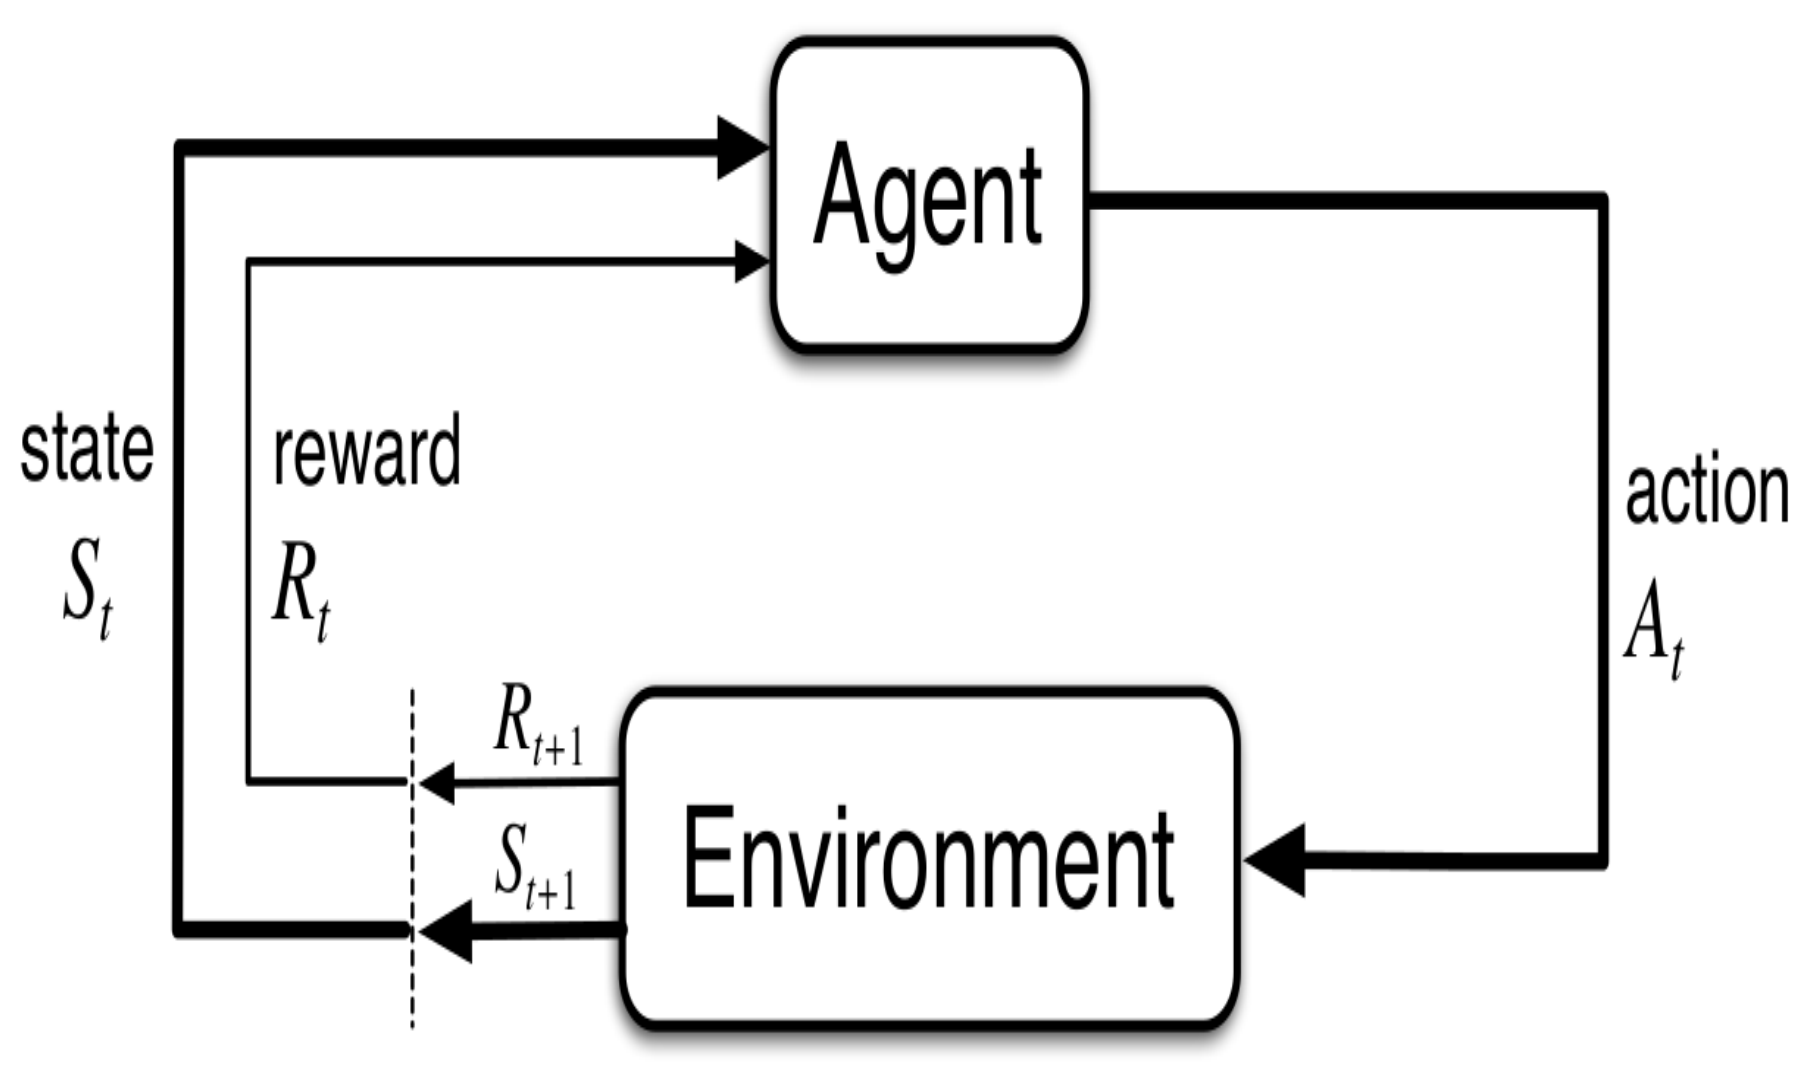
\includegraphics[width=0.5\linewidth]{MDP Framework.png}

The components of this framework at:
\begin{itemize}
    \item The Agent and the Environment interact in a time-sequenced loop.
    \item Agent responds to the [State, Reward] by taking an Action
    \item Environment responds by producing the next step's random State
    \item Environment produces a random scalar denoted as Reward
    \item Each State is assumed to have the Markov Property, meaning:
    \begin{itemize}
        \item Next State/Rewardd depends only on the current States
        \item Current State captures all the relevant information from the history
        \item Current State is sufficient statistic of the future
    \end{itemize}
    \item The goal of the agent is to maximize the Expected Sum of all future Rewards
    \item This is done by controlling the (Policy: State $\rightarrow$ Action) function
    \item This is a dynamic system under uncertainty
\end{itemize}

Formally this framework becomes:
The following notation is for discrete time steps. Continuous-time formulation is analogous (often involving Stochastic Calculus)
\begin{itemize}
    \item Time steps denoted as $t=1,2,3, \ldots$
    \item Markov States $S_t \in \mathcal{S}$ where $\mathcal{S}$ is the State Space
    \item Actions $A_t \in \mathcal{A}$ where $\mathcal{A}$ is the Action Space
    \item Rewards $R_t \in \mathbb{R}$ denoting numerical feedback
    \item Transitions $p\left(r, s^{\prime} \mid s, a\right)=\mathbb{P}\left[\left(R_{t+1}=r, S_{t+1}=s^{\prime}\right) \mid S_t=s, A_t=a\right]$
    \item $\gamma \in[0,1]$ is the Discount Factor for Reward when defining Return
    \item Return $G_t=R_{t+1}+\gamma \cdot R_{t+2}+\gamma^2 \cdot R_{t+3}+\ldots$
    \item Policy $\pi(a \mid s)$ is probability that Agent takes action $a$ in states $s$
    \item The goal is find a policy that maximizes $\mathbb{E}\left[G_t \mid S_t=s\right]$ for all $s \in \mathcal{S}$
\end{itemize}

\paragraph*{Difficulties of MDP problems}
These problems are hard because they have can have large and complex state and action spaces, with limited or no direct feedback on the correctness of the Action, only on the Reward earnt. 
In addition to this there is significant time-sequenced complexity, involving delayed consequences of actions. 
Furthermore, Agents rarely know the model of the Environment (i.e. the state transition probabilities and rewards). Thus, Agents have to learn the model and solve for the Optimal Policy. 

\paragraph*{Value Function and the Bellman Equation}
Under the policy $\pi$ we have the value function $V^\pi(s)=\mathbb{E}\left[G_t \mid S_t=s\right] \text { for all } s \in \mathcal{S}$ i.e.,
$$
V^\pi(s)=\sum_a \pi(a \mid s) \sum_{r, s^{\prime}} p\left(r, s^{\prime} \mid s, a\right) \cdot\left(r+\gamma V^\pi\left(s^{\prime}\right)\right) \text { for all } s \in \mathcal{S}
$$
This results in an Optimal Value Function $V^*(s)=\max _\pi V^\pi(s)$ for all $s \in \mathcal{S}$:
$$
V^*(s)=\max _a \sum_{r, s^{\prime}} p\left(r, s^{\prime} \mid s, a\right) \cdot\left(r+\gamma V^*\left(s^{\prime}\right)\right) \text { for all } s \in \mathcal{S}
$$
There exists an Optimal Polixy $\pi^*$ achieving $V^*(s)$ for all $s \in S$. We determing $V^\pi(s)$ with Prediction and $V^*(s)$ with Control. The recursive equation written above ar ethe Bellman Equations (with the continuous time equivalents being the Hamiltonian-Jacobi-Bellman (HJB) equations). The algorithms based on Bellman equations are broadly classified as either:
\begin{itemize}
    \item Dynamic Programming
    \item Reinforcement Learning
\end{itemize}

\paragraph*{Dynamic Programming}
When the Probability Model of the Environment is known we can use Dynamic Programming, these algorithms take advantage of the knowledge of probabilities, as such they do not required interaction with the environment (i.e. a Planning Algorithm in AI terminology).
DP algorithms are iterative algorithms based on Fixed-Point Theorem, i.e. finding a Fixed Point of an Operator based on the Bellman Equation. 
DP is not effective in practive due to the curse of Dimensionality and the curse of Modelling. 
There are some known solutions to the curse of Dimensionality (Approximate DP), but to solve both effectively we need to utilise RL.

\paragraph*{Reinforcement Learning}
Since we don't typically have access to the Environments Probability Model, we use RL to learn it. We usually have access to the individual transitions of the Environment. RL interacts with either the actual or simulated environment, recieving individual transitions to the next State/Reward (i.e. a trail and error approach linking actions to returns). 

\end{document}